\section{Evaluation of the modelled response to ENSO}
\label{sec:model-val}

Before turning to the main processes responsible for the modelled response of epipelagic communities to ENSO (next sections), we first evaluate the ability of the physical, biogeochemical and biological models we use to reproduce ENSO-related fluctuations. Past literature already demonstrated the ability of NEMO/PISCES model to reproduce many aspects of physical (e.g., \citealt{vialardModelStudyOceanic2001, lengaigneMechanismsControllingWarm2012, drushkaProcessesDrivingIntraseasonal2015, puyModulationEquatorialPacific2019}) and biogeochemical (e.g., \citealt{ masottiLargescaleShiftsPhytoplankton2011,gorguesRevisitingNina19982010, martinezReconstructingGlobalChlorophylla2020}) response to ENSO in the tropical Pacific. In the following subsection, we briefly demonstrate the ability of our simulation to capture the ENSO-related signals that are important to marine ecosystems, namely surface temperature (which modulates the functional response to prey as well as all the metabolic rates controlling growth, reproduction, development, maintenance and swimming speed in APECOSM), sea-level anomalies (a proxy of the thermocline depth, which modulates vertical habitats of epipelagic species), surface currents (which passively transport simulated biomass) and chlorophyll concentration anomalies that is at the base of food chains.

\subsection{Physical response}

 Figure \ref{fig:nemo-had-sst}a-c first allows to evaluate the ability of our simulation to reproduce the ENSO signature in sea surface temperature (SST). Figure \ref{fig:nemo-had-sst}a presents the temporal evolution of ENSO as observed and simulated by the model from the Oceanic Niño Index (hereafter ONI) \footnote{\url{https://www.cpc.ncep.noaa.gov/data/indices/oni.ascii.txt}}, computed from a 3-month running mean of SST anomalies averaged over the Niño 3.4 region (5N-5S, 170W-120W). Over the entire period considered (1958-2018), the ONI index exceeds 2\degree{}C on three occasions corresponding to the three most intense El Niño events observed in 1982/83, 1997/98 and 2015/16. Other more moderate El Niño events are also observed in 1986/87, 1991/92, 2002/03 and 2009/2010, with ONI values ranging between 1\degree{}C and 2\degree{}C. Major La Niña events are observed in 1970/71, 1973/74, 1988/89, 1999/2000 and 2007/08 and 2010/11. This panel also reveals that the model is able to accurately simulate the timing and amplitude of ENSO events, as shown by the significant correlation (0.92) between observed and modeled ONI indices at the $95\%$ level of confidence (based on Student's t-test with an effective number of degrees of freedom that is corrected based on the 1-lag autocorrelation of each time-series, as reported in \citealp{brethertonEffectiveNumberSpatial1999}). Despite this general agreement, the model tends to overestimate the amplitude of the strongest El Niño events. 

\begin{figure}[h!tp]
	\centering
	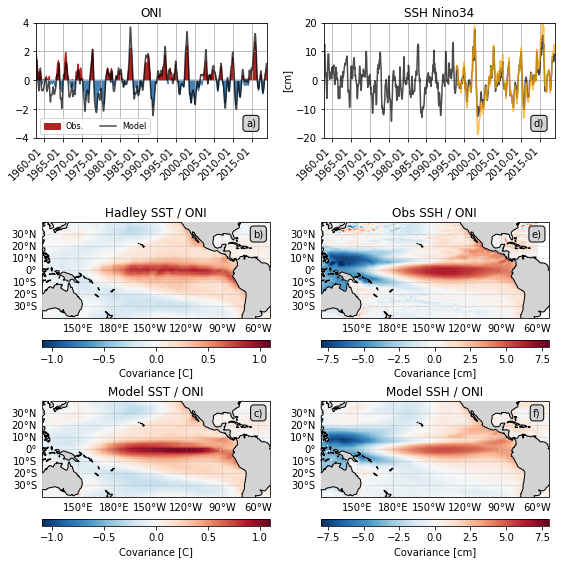
\includegraphics[scale=0.6]{figs/fig1.png}
	\caption{Time evolution of the ONI index for observations and model over the period 1958-2018 (a). ENSO-related SST patterns for observations \citep{raynerGlobalAnalysesSea2003} (b) and model (c) derived from covariance maps of detrended monthly SST anomalies onto the ONI index over the 1958-2018 period. Time evolution of zonal surface current anomalies over the Niño34 region for observations over the 1993-2018 period \citep{rioGOCEOceanCirculation2014} and model over the 1958-2018 period (d). ENSO-related sea-level and ocean current patterns for observations (e) and model (f) derived from covariance maps of detrended monthly sea-level and current anomalies onto the ONI index over the period 1993-2018. The dashed box represents the Niño34 region used for averaging.}
	\label{fig:nemo-had-sst}
\end{figure}

Figure \ref{fig:nemo-had-sst}bc then illustrates the typical SST spatial patterns associated with ENSO for both the observations (HadISST1, \citealp{raynerGlobalAnalysesSea2003}) and model, extracted from the covariance maps of detrended monthly SST anomalies onto the ONI index. The observed and modelled SST patterns are very similar and are characterized by warm SST anomalies (1\degree{}C) located in the central and eastern equatorial Pacific, flanked by the traditional horseshoe cooling pattern in the western Pacific that extends into the northern and southern subtropical Pacific.    


ENSO-induced SST variations are known to be strongly related to variations in ocean current and sea level (a proxy for thermocline depth), with SST signals largely driven by vertical displacement of the equatorial thermocline in response to equatorial wind variations. Figure \ref{fig:nemo-had-sst}d illustrates the temporal evolution of zonal current anomalies averaged over the Niño34 region for observations\footnote{\url{https://doi.org/10.48670/moi-00050}} (\citealp{rioGOCEOceanCirculation2014}) available from 1993 to present and the model. The model faithfully reproduces the observed anomalies (significant correlation of 0.89), with eastward currents anomalies during El Niño events (reaching 0.7 m.s-1 at the peak of the 1982/83 and 1997/98 events) and westward currents anomalies during La Niña events. As shown in Figure \ref{fig:nemo-had-sst}e, these easterly current anomalies during El Niño are heard over the entire equatorial Pacific between 2N and 5S, a spatial structure well captured by the model (Fig. \ref{fig:nemo-had-sst}f).
%from the DUACS multi-mission altimeter data \footnote{\url{https://doi.org/10.48670/moi-00148}}. The temporal evolution of observed sea level anomalies matches very well the observed SST evolution over the same region (Fig \ref{fig:nemo-had-sst}a), both being correlated at ?.??: the deepening of the thermocline observed in the central and eastern Pacific during El Niño events in response to westerly wind anomalies indeed contribute to El Niño warming by limiting the amount of cold waters brought to the surface, the opposite occurring during La Niña events.  The model accurately reproduces the observed sea level evolution (Fig \ref{fig:nemo-had-sst}d), with a correlation coefficient reaching 0.94 (significant at the $95\%$ level of confidence). 
With respect to sea-level observed\footnote{\url{https://doi.org/10.48670/moi-00148}} its observed signature related to ENSO (Fig. \ref{fig:nemo-had-sst}e) is characterized by a shoaling of the thermocline in the western Pacific (negative sea level anomalies) and a deepening in the central and eastern Pacific (positive sea level anomalies), a signal which is physically consistent with the cooling observed in the west and the warming in the east (Fig. \ref{fig:nemo-had-sst}b). As shown on Figure \ref{fig:nemo-had-sst}f, the model captures this zonal sea-level seesaw very accurately.

\subsection{Biogeochemical response}

Figure \ref{fig:nemo-had-sst}a-c then assesses the ability of our simulation to capture ENSO-related variability of cholorophyll concentration, an indicator of the concentration of low-trophic level organisms that are at the base of the marine food chain. To this end, we compare simulated chlorophyll concentrations with observation-based estimates derived from the multi-satellite monthly OceanColour-CCI V5 CHL-a dataset\footnote{\url{http://dx.doi.org/10.5285/1dbe7a109c0244aaad713e078fd3059a}} \citep{sathyendranathOceanColourTimeSeries2019} available over the 1997-09/2018-12 period. 
%This high resolution (4 km)  dataset is regridded on a regular $1\times 1$ grid by computing weighted chlorophyll averages over $24\times24$ boxes, with the weights being provided by the cosine of latitude. When more than $1/3$ of the data used in the averaging is missing, the regridded cell is masked.

\begin{figure}[h!tp]
	\centering
	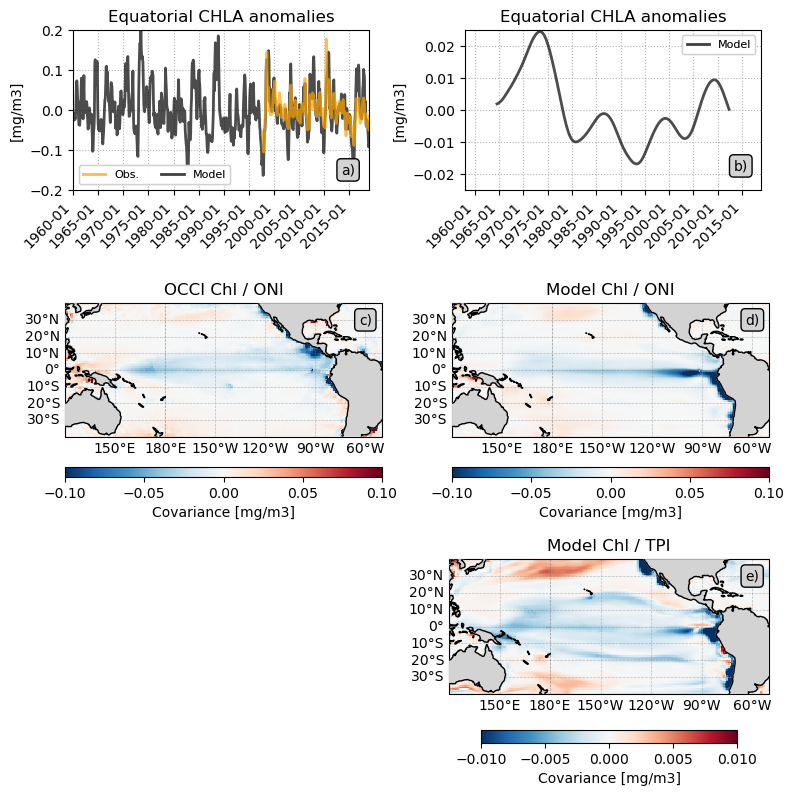
\includegraphics[scale=0.4]{figs/fig2.png}
	\caption{Time evolution of interannual surface chlorophyll anomalies in the equatorial Pacific for observations over the period 1998-2018 (yellow curve) and  model over the period 1960-2018 (black curve) (a). Covariance between the chlorophyll anomalies and the ONI indexover the period 1998-2018 for observations (b) and model (c). The dashed frame represents the equatorial region used in the averaging.}
	\label{fig:nemo-sat-chl}
\end{figure}

Figure \ref{fig:nemo-sat-chl}a shows the temporal evolution of chlorophyll anomalies averaged over the equatorial Pacific for the model and observations. In agreement with past literature, El Niño events are associated with a decrease in chlorophyll all along the equator (Fig. \ref{fig:nemo-sat-chl}a) in response to the combined action of the nutricline deepening in the eastern Pacific and eastward advection of nutrient‐poor waters by anomalous eastward currents in the western and central Pacific. The reverse occurs during La Niña events. As a result, equatorial chlorophyll anomalies are strongly anti-correlated with variations in Niño34 SST (R=-0.74) and sea level (R=-0.78). The model faithfully reproduces these observed chlorophyll variations, with a correlation coefficient reaching $0.80$ (significant at the $95\%$ level of significance).

Figure \ref{fig:nemo-sat-chl}bc show the typical spatial patterns of surface chlorophyll anomalies associated with ENSO for the observations and the model over their common period. In agreement with \ref{fig:nemo-sat-chl}a, El Nino leads to a decrease in chlorophyll concentration along the equator east of 150\degree{}E. Despite an overestimation of the modeled chlorophyll decrease in the eastern Pacific, the observations (upper panel) and the model (lower panel) show similar patterns. Note that recalculating the simulated spatial pattern over the entire modeled period (1958-2018) does not significantly alter the results (not shown). 

\subsection{Ecosystem response}

In this section, we compare the evolution of simulated epipelagic biomass to available observations in the equatorial Pacific. As mentioned in the introduction, the largest observational inter-annual dataset pertaining to high trophic level marine organisms in the equatorial Pacific is based on tuna catches. Here we use monthly catch of skipjack and yellowfin tuna by purse seiners provided at 1° and 5° spatial resolution by the Western and Central Pacific Fisheries Commission (WCPFC) and processed by the French National Research Institute for Sustainable Development (IRD)\footnote{\url{https://doi.org/10.5281/zenodo.1164128}}, as described in  \citep{taconetGlobalMonthlyCatch2018}. We first extract skipjack and yellowfin purse-seine catches from the raw input file. We then discard observations with a temporal resolution greater than one month and data for which the geographical coordinates are not referenced in the database. The remaining observations are finally binned onto on a regular $1 \times 1$ grid. The final product consists of monthly maps of tuna catches covering the 1959-2018 period. However, due to the limited spatial coverage of the purse-seine fleets in the early part of the record, we only analyse this dataset from 1985 onwards. We compare catch observations to the biomass of the epipelagic community integrated from 30cm to 70cm, the typical size range of  skipjack and yellowfin tunas caught by purse seiners in this region. In making this comparison, it should be kept in mind that fishing data do not result from a random sampling of the ocean. They are indeed influenced by both climate variability and the numerous socio-economic factors controlling dynamics and distribution of fishing effort. Furthermore, although tuna represent the majority of the epipelagic biomass in this size range in this region, our model does not explicitly simulate specific tuna species but generic oceanic communities such as the epipelagic community we study here.
% Therefore, these data  highly biased estimators of the actual biomass of fish swimming in the ocean that are 

\begin{figure}[h!tp]
	\centering
	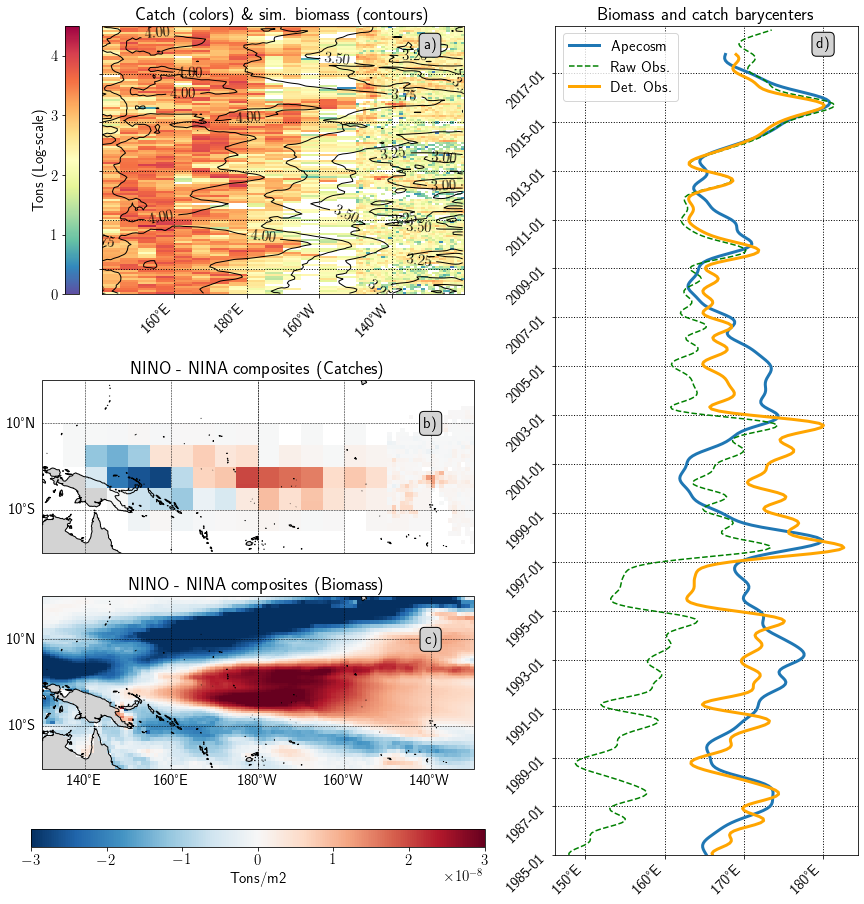
\includegraphics[scale=0.35]{figs/plot_validation_apecosm.png}
	\caption{Time-longitude diagram of observed catches (colors, log-scale in Tons) and simulated epipelagic biomass (contours, log-scale in Tons) cumulated between 10N and 10S (a). Difference between El Nino and La Nina composites over the period 2007-2018 for observed catches (b) and simulated epipelagic biomass (c) . Temporal evolution of the barycenters over the period 1985-2018 of simulated epipelagic biomass (black), observed catches (blue) and detrended observed catches (yellow) (d).}
	\label{fig:apecosm_validation}
\end{figure}

Figure \ref{fig:apecosm_validation}a shows the longitude-time diagram of observed catches integrated between 10N and 10S over the period 2008-2018. It shows significant variations in the zonal extent of tuna catches in the equatorial Pacific. These catches are indeed confined to the west of the dateline during certain periods such as in 2008 and 2011, when La Niña conditions prevail over the Pacific. In contrast, these catches extends eastward into the central Pacific for other periods such as 2009-2010 and 2014-2016, characterized by El Niño conditions. Despite the different nature of observed catches and our modeled epipelagic biomass, the evolution of the zonal extension of the modeled biomass compares surprisingly well with that of the tuna catches over the recent period: the La Niña events of 2008 and 2011 are indeed characterized by a westward retraction of the epipelagic biomass, while the El Niño periods of 2009-2010 and 2014-2016 are characterized by a clear eastward extension of the epipelagic biomass. Figure \ref{fig:apecosm_validation}bc show a composite difference between the observed catches and simulated biomass for El Niño (2009-10/2010-03, 2014-10/2015-03, 2015-10/2016-03) and La Niña conditions (2007-10/2008-03, 2008-10/2009-03, 2010-10/2011-03, 2011-10/2012-03). It illustrates the typical east-west shift pattern that is associated with ENSO in the recent period. Observed catches increase in the central and eastern Pacific and decrease in the Western Pacific between La Niña to El Niño conditions, consistent with an eastward shift of the epipelagic biomass. Observed catches and simulated biomass composites show similar patterns, although slightly shifted westward in the model.

To assess the agreement between observations and model over a longer period, Figure \ref{fig:apecosm_validation}d shows the longitude of the barycenters of observed tuna catch and modeled biomass over the period 1985-2018. Consistent with the good agreement between model and observations presented in Fig\ref{fig:apecosm_validation}a, the evolution of model and observed barycenters matches well over the recent period considered (2008-2018), with a correlation of 0.68 between the two time series: this is particularly the case for the 2014-2016 El Niño sequence, where both model and observations indicate an eastward shift of the barycenter, from 160°E in early 2014 to 180°W in early 2016, before retracting westward after that date. Looking at the observations over the entire observational record, the most striking feature is a gradual eastward shift in the location of the catches barycenter from 155°E in the 80's to 170°E in the last decade. This trend is probably related to the progressive increase in power of fishing vessels, which allows them to move further away from their home ports, mostly located in the western Pacific. In addition to this low frequency trend, higher frequency variations are also evident, especially during the 1986/87, 1997/98 or 2001/02 El Niño events, where observed catches shift eastwards. In order to eliminate this low-frequency trend and to make a fair comparison with the model outputs, we smoothed and detrended the time series of the longitude of the observed catch barycenter (yellow curve on Figure \ref{fig:apecosm_validation}b). The time series of the model and detrended observations show a reasonable match over the whole period, with a correlation of 0.45. The strong correlation coefficient existing between ONI timeseries and model biomass barycenter (0.74) as well as observed catches barycenter (0.52) further demonstrates the control exerted by ENSO in both observations and model. While observations and model generally show a westward shift during La Niña conditions and an eastward shift during El Niño conditions, these time series deviate from each other during specific periods, such as the strong La Niña of 1999/2000, which is characterized by a stronger westward retraction in the model or during the warm years of 2003-2005 with the barycenter of observed catches shifting westward relative to that of the modeled biomass.

In summary, the analyses shown above illustrate the ability of the various components of the model to accurately reproduce the physical, biogeochemical and ecosystem response to ENSO. Specifically, the ecosystem model simulate zonal migrations of large epipelagic communities in the equatorial Pacific in response to ENSO in a manner similar to that observed for tuna catches. This reasonable agreement indicates that our ecosystem simulation is a relevant tool to study the processes responsible for the response of epipelagic community to ENSO. In what follows, the results are detailed for three selected size classes: 3 cm, representing small epipelagic fishes, 20 cm, representing intermediate sizes, and 90 cm, representing large individuals. The latter two are representative of the lower and upper limits of the size range of tuna exploited by purse seiners in the region.

\clearpage